% !TeX root = ../../main.tex
\subsection{Visual Programming Scalability}%
\label{sec:related.ad.vpl-scalability}

\Ac{VPL}-based approaches suffer from disproportionate scalability issues
between the code and the respective model's
complexity~\cite{Leitao:2013:PESLGD}.

As an example, consider the Irina Viner-Usmanova \ac{RGC}.
\Cref{fig:related.ad.vpl-scalability.rgc} depicts an outside view of the
\ac{RGC} and its prominent overarching roof covering, the latter conceived using
Grasshopper.  Developing a roof covering with such a contour lends itself well
to \ac{AD}.

Such complex \ac{AD} projects tend to require complex \ac{AD} programs that
become overly difficult to develop and understand with \acp{VPL}.  This
disadvantage, however, is mitigated by \ac{TPL} alternatives which, despite
project complexity, scale relatively better than \acp{VPL} on account of
abstraction mechanisms.

\begin{figure}[htbp]
  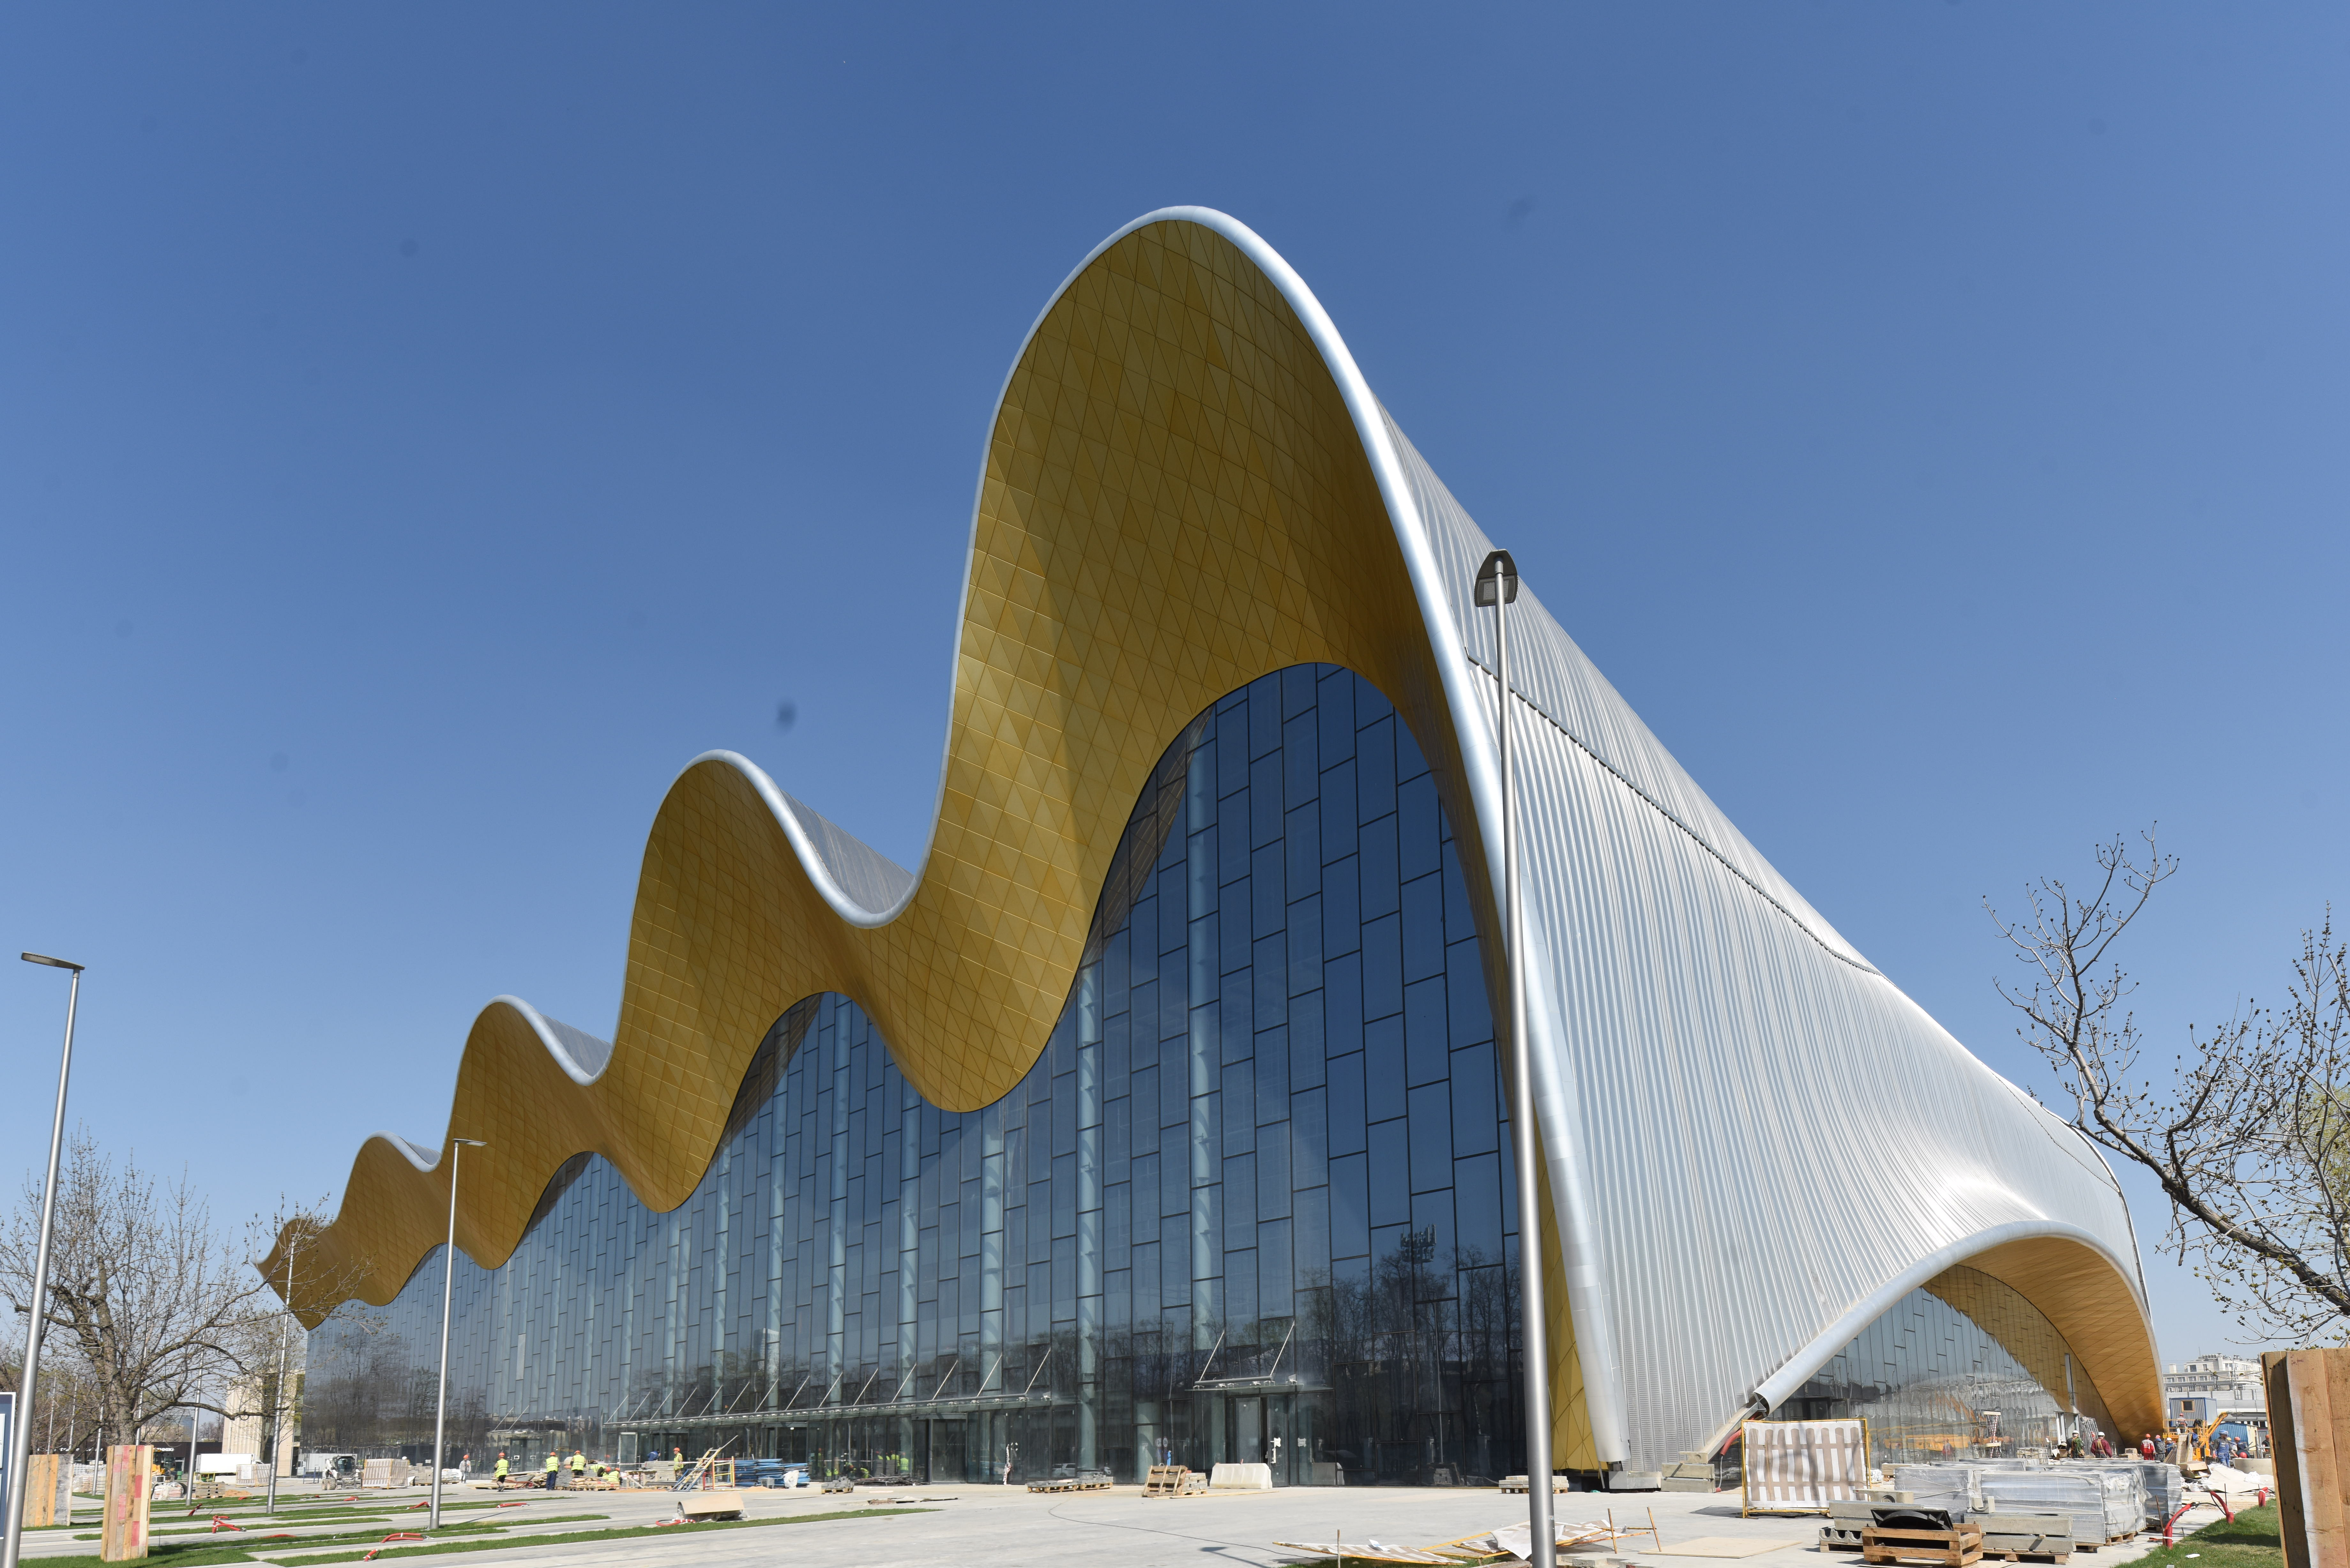
\includegraphics[width=\linewidth]{fig/rgc}
  \begin{minipage}{\linewidth}
  \scriptsize Source:
  \url{https://www.grasshopper3d.com/photo/rhythmic-gymnastics-center-moscow-russia-5}
  \end{minipage}
  \caption{\label{fig:related.ad.vpl-scalability.rgc}
    Irina Viner-Usmanova \ac{RGC}, Moscow, Russia.}%
\end{figure}
